\clearpage







\section{Abstract}


\subsubsection{One or two sentences providing a basic introduction to the field}
% comprehensible to a scientist in any discipline.
\lettr{W}rite abstract here.


\subsubsection{Two to three sentences of more detailed background}
% comprehensible to scientists in related disciplines.


\subsubsection{One sentence clearly stating the general problem (the gap)}
% being addressed by this particular study.


\subsubsection{One sentence summarising the main result}
%  (with the words “here we show” or their equivalent).


\subsubsection{Two or three sentences explaining what the main result reveals in direct comparison to what was thought to be the case previously}
% or how the main result adds to previous knowledge


\subsubsection{One or two sentences to put the results into a more general context.}



\subsubsection{Two or three sentences to provide a broader perspective, }
% readily comprehensible to a scientist in any discipline.



%%%%%%%%%%%%%%%%%%%%%%%%%%%%%%%%%%%%%%%%%%%%%%%%%%%%%%%%%%%%%%%%%%%%%%%%%%%%%%%%%%%%%%%%%%%%%%%%%%%%%%%%%%%%%%%%%%%%%%%%%%%%%%%%%%%%%%%%%%%%%%%%%%%%%%%%%%%

\clearpage
\section{Introduction}

%%%%%%%%%%%%%%%%%%%%%%%%%%%%%%%%%%%%%%%%%%%%%%%%%%%%%%%%%%%%%%%%%%%%%%%%%%%%%%%%%%%%%%%%%%%%%%%%%%%%%%%%%%%%%%%%%%%%%%%%%%%%%%%%%%%%%%%%%%%%%%%%%%%%%%%%%%%





%%%%%%%%%%%%%%%%%%%%%%%%%%%%%%%%%%%%%%%%%%%%%%%%%%%%%%%%%%%%%%%%%%%%%%%%%%%%%%%%%%%%%%%%%%%%%%%%%%%%%%%%%%%%%%%%%%%%%%%%%%%%%%%%%%%%%%%%%%%%%%%%%%%%%%%%%%%

\clearpage
\section{Methods}

%%%%%%%%%%%%%%%%%%%%%%%%%%%%%%%%%%%%%%%%%%%%%%%%%%%%%%%%%%%%%%%%%%%%%%%%%%%%%%%%%%%%%%%%%%%%%%%%%%%%%%%%%%%%%%%%%%%%%%%%%%%%%%%%%%%%%%%%%%%%%%%%%%%%%%%%%%%

To measure pathogen richness I used data from \cite{luis2013comparison}. 
These simply include known infections of a bat species with a pathogen species. 
Only species with at least one pathogen were included in the analysis.
To control for study bias I collected the number of pubmed and scholar citations for each bat species including synonyms from ITIS \cite{itis} via the taxize package \cite{chamberlain2013taxize}.
The counts were scraped using the rvest package \cite{rvest}.






I used two measures of population structure. 
$F_{ST}$ and the number of subspecies.
The number of of subspecies was counted using the Wilson and Reeder taxonomy \cite{wilson2005mammal}.

\begin{knitrout}\footnotesize
\definecolor{shadecolor}{rgb}{0.969, 0.969, 0.969}\color{fgcolor}\begin{kframe}


{\ttfamily\noindent\bfseries\color{errorcolor}{\#\# Error in mget(words, envir, "{}any"{}, NA, inherits = TRUE): cannot open file '/home/tim/Dropbox/phd/Documents/thesis/.Ch3Cache/wilsonReaderTaxonomyRead\_949262de95271ee1f5068b4e7140b466.rdb': No such file or directory}}

{\ttfamily\noindent\bfseries\color{errorcolor}{\#\# Error in eval(expr, envir, enclos): cannot open file '/home/tim/Dropbox/phd/Documents/thesis/.Ch3Cache/wilsonReaderTaxonomyRead\_949262de95271ee1f5068b4e7140b466.rdb': No such file or directory}}

{\ttfamily\noindent\bfseries\color{errorcolor}{\#\# Error in eval(expr, envir, enclos): cannot open file '/home/tim/Dropbox/phd/Documents/thesis/.Ch3Cache/wilsonReaderTaxonomyRead\_949262de95271ee1f5068b4e7140b466.rdb': No such file or directory}}\end{kframe}
\end{knitrout}











Measures of body mass are taken from Pantheria \cite{jones2009pantheria}.
They are log transformed due to the strong right skew.


































%Pubmed was scraped on pubmedScrapeDate and Google Scholar was scraped on scholarScrapeDate

To control for phylogenetic nonindependance I used the best-supported phylogeny from \cite{fritz2009geographical} which is the supertree from \cite{bininda2007delayed} with names updated to match the Wilson \& Reeder taxonomy \cite{wilson2005mammal}.
Phylogenetic manipulation was performed using the ape package \cite{ape}.




\begin{knitrout}\footnotesize
\definecolor{shadecolor}{rgb}{0.969, 0.969, 0.969}\color{fgcolor}\begin{figure}[t]

{\centering 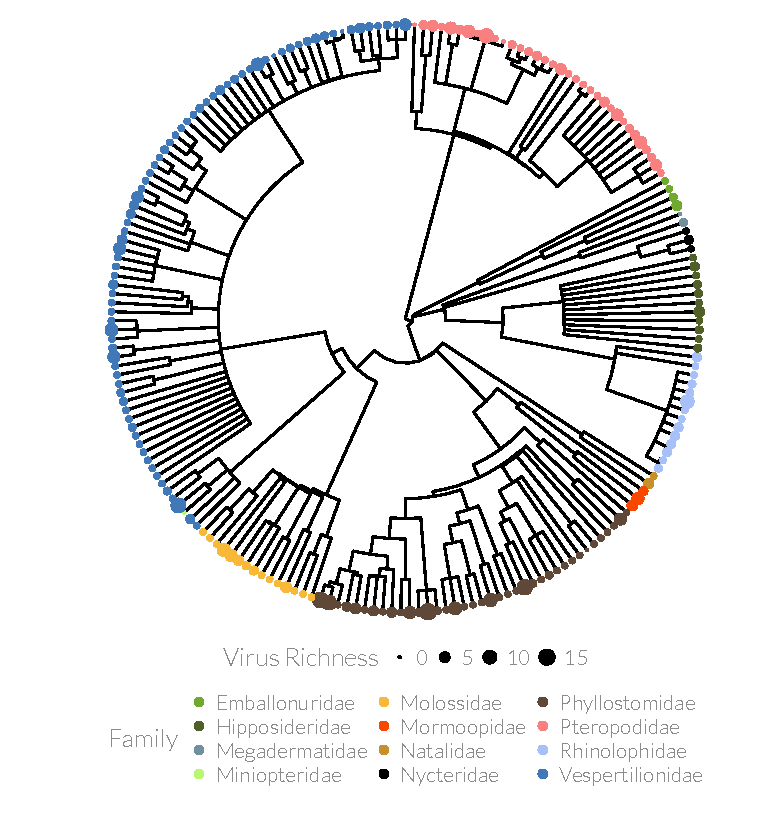
\includegraphics[width=0.8\textwidth]{figure/treePlot-1} 

}

\caption[Pruned phylogeny with dot size showing number of pathogens and colour showing family]{Pruned phylogeny with dot size showing number of pathogens and colour showing family.}\label{fig:treePlot}
\end{figure}


\end{knitrout}






I wanted to run three models using the phylolm package testing the relationship between pathogen richness and log number of subspecies.
I tried phylogenetically controlled, multivariate GLMs with poisson errors and identity links.
This model was fitted both with and without an interaction term between number of subspecies and study effort.
I also fitted a phylogenetically controlled, GLM with poisson errors and identity link to pathogen richness and study effort.
The residuals from this model was then used as the response variable in a multivariate GLM.
However, with these models the numerical optimisation failed to converge.

I ran three models using the caper package \cite{caper} testing the relationship between pathogen richness and log number of subspecies.
All independant variables were log transformed --- study effort was $\log(\text{citations} + 1)$.
I ran phylogenetically controlled, multivariate linear models.
This model was fitted both with and without an interaction term between number of subspecies and study effort.
We also fitted a phylogenetically controlled, GLM with poisson errors and identity link to pathogen richness and study effort.
The residuals from this model was then used as the response variable in a multivariate GLM.




\clearpage











\clearpage


These are the fits from models fitted with the species with only 1 virus species removed.
We can see that if number of subspecies is unlogged, it remains marginally significant.
If subspecies is logged it is no longer significant.




\begin{knitrout}\footnotesize
\definecolor{shadecolor}{rgb}{0.969, 0.969, 0.969}\color{fgcolor}\begin{figure}[t]

{\centering 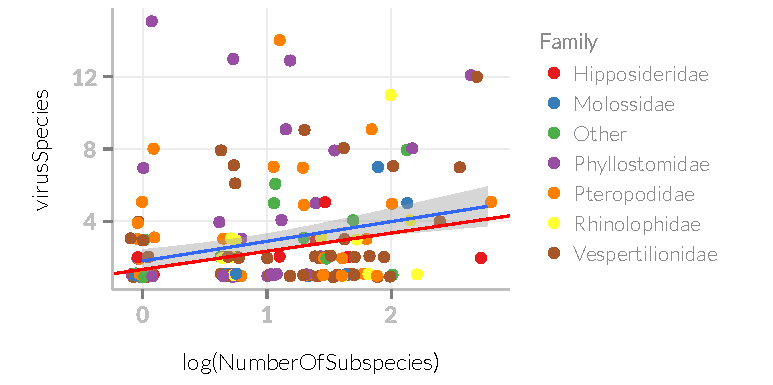
\includegraphics[width=0.8\textwidth]{figure/plotSubspecies-1} 

}

\caption[Number of virus species against log number of subspecies]{Number of virus species against log number of subspecies. Nonphylogenetic trend line in blue. Phylogenetic model (evaluated at mean body mass and mean study effort values) is shown in red.}\label{fig:plotSubspecies}
\end{figure}


\end{knitrout}







\begin{knitrout}\footnotesize
\definecolor{shadecolor}{rgb}{0.969, 0.969, 0.969}\color{fgcolor}\begin{figure}[t]

{\centering 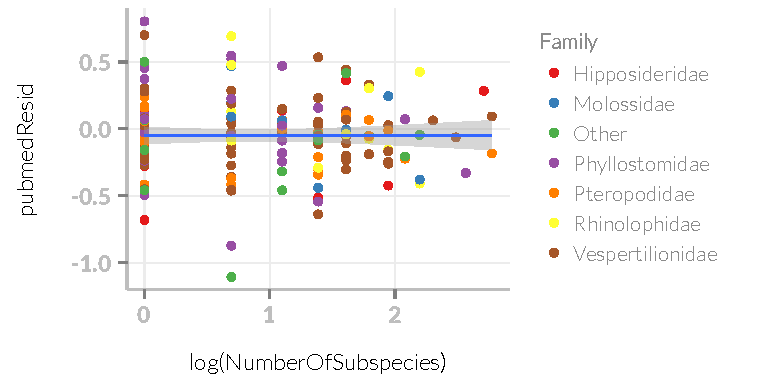
\includegraphics[width=0.8\textwidth]{figure/pubmedresidPlot-1} 

}

\caption[Plot using residuals from number of viruses against number of citations (study effort)]{Plot using residuals from number of viruses against number of citations (study effort). Nonphylogenetic trend line added. }\label{fig:pubmedresidPlot}
\end{figure}


\end{knitrout}

%%%%%%%%%%%%%%%%%%%%%%%%%%%%%%%%%%%%%%%%%%%%%%%%%%%%%%%%%%%%%%%%%%%%%%%%%%%%%%%%%%%%%%%%%%%%%%%%%%%%%%%%%%%%%%%%%%%%%%%%%%%%%%%%%%%%%%%%%%%%%%%%%%%%%%%%%%%

\clearpage
\section{Results}

%%%%%%%%%%%%%%%%%%%%%%%%%%%%%%%%%%%%%%%%%%%%%%%%%%%%%%%%%%%%%%%%%%%%%%%%%%%%%%%%%%%%%%%%%%%%%%%%%%%%%%%%%%%%%%%%%%%%%%%%%%%%%%%%%%%%%%%%%%%%%%%%%%%%%%%%%%%

See Figure \ref{fig:plotSubspeciesCoefs} for a display of estimated coefficients for the two models using number of viruses as the response variable. 
The main model with mass, study effort and number of subspecies as predictors found study effort to be highly significant ($\beta = $1.01, $p = $\ensuremath{3.9\times 10^{-12}}). 
The number of subspecies was marginally significant ($\beta = $ 0.48, $p = $0.06). 
The effect of nonindependance due to phylogeny was very small ($\lambda = $0.07, $p = $0.1).

The interaction term between study effort and number of subspecies, when included, was not significant ($\beta = $ 0.23, $p = $0.12).

The model using the residuals from a regression between number of viruses and study effort as the response variable found no significant affect of number of subspecies. 
Mass was marginally significant.




\begin{knitrout}\footnotesize
\definecolor{shadecolor}{rgb}{0.969, 0.969, 0.969}\color{fgcolor}\begin{figure}[t]

{\centering 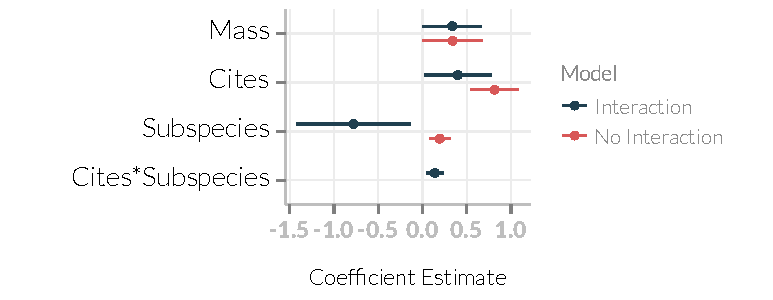
\includegraphics[width=0.8\textwidth]{figure/plotSubspeciesCoefs-1} 

}

\caption[
Plot of coefficient estimates and 95\% confidence intervals for phylogenetic model with (inter) and without (joint) interactions between study effort and number of subspecies]{
Plot of coefficient estimates and 95\% confidence intervals for phylogenetic model with (inter) and without (joint) interactions between study effort and number of subspecies. 
Without interactions, number of subspecies is marginally significant.
}\label{fig:plotSubspeciesCoefs}
\end{figure}


\end{knitrout}










%%%%%%%%%%%%%%%%%%%%%%%%%%%%%%%%%%%%%%%%%%%%%%%%%%%%%%%%%%%%%%%%%%%%%%%%%%%%%%%%%%%%%%%%%%%%%%%%%%%%%%%%%%%%%%%%%%%%%%%%%%%%%%%%%%%%%%%%%%%%%%%%%%%%%%%%%%%

\clearpage
\section{Discussion}  

%%%%%%%%%%%%%%%%%%%%%%%%%%%%%%%%%%%%%%%%%%%%%%%%%%%%%%%%%%%%%%%%%%%%%%%%%%%%%%%%%%%%%%%%%%%%%%%%%%%%%%%%%%%%%%%%%%%%%%%%%%%%%%%%%%%%%%%%%%%%%%%%%%%%%%%%%%%









